This appendix follows Uranga's. It has the purpose of introducing some useful concepts of group theory and their application. It is by no means complete and formal.

%******************** LIE GROUPS AND LIE ALGEBRA *********************
\section{Lie Groups and Lie Algebra}
\paragraph{Lie Groups}
A \emph{Lie Group} $G$ is a group where the elements are labeled by a set of continuous real parameters $\xi^a$, $a = 1 \dots N$, such that
\begin{equation}
    g(\xi) \cdot g(\xi') = g(f(\xi,\xi')),
\end{equation}
where $f^a(\xi,\xi')$ is a continuous function of $\xi,\xi'$. A Lie group is also a differentiable manifold, with $g(\xi=0)=e$, and dimension $\dim{G} = N$.

\paragraph{Group Representations}
A representation is a map $R$ from the group $G$, onto the endomorphisms on a vector space $V$, $\End(V)$, such that each element $g \in G$ is represented by an operator $R(g)$ acting on V and it preserves the group properties, that it
\begin{equation}
\begin{aligned}
    R: G &\to \End(V),  \quad \textup{s.t.} \, R(g \cdot h) = R(g)R(h)\\
       g &\mapsto R(g)
\end{aligned}
\end{equation}
Let $\ket{e_i}$ be a basis of $V$. Then, the matrix elements of $R(g)$ are
\begin{equation}
    R(g)_{ij} = \bra{e_i} R(g) \ket{e_j}.
\end{equation}
A representation is called \emph{reducible} if can be decomposed into block-diagonal form
\begin{equation}
     R(g) = \begin{pmatrix}
        R_1(g) & 0 \\
        0 & R_2(g)
    \end{pmatrix}, \quad \forall g \in G .
\end{equation}

Let's consider two representation spaces $V_1$ and $V_2$, with dimensions $n_1$ and $n_2$ and basis $\ket{e_i}$ and $\ket{f_n}$, respectively. Further, let's consider the representations $R_1: G \to \End(V_1)$ and $R_2: G \to \End(V_2)$. We can define the \emph{direct sum of representations} $R = R_1 \oplus R_2$, of dimension $\dim(R) = n_1 + n_2$, by
\begin{equation}
\begin{aligned}
    R = R_1 \oplus R_2 : G &\to \End(V_1 \oplus V_2) \\
    g &\mapsto R(g) = \begin{pmatrix}
        R_1(g) & 0 \\
        0 & R_2(g)
    \end{pmatrix}
\end{aligned}
\end{equation}
and the \emph{tensor product of representations} $R = R_1 \otimes R_2$, of dimension $\dim(R) = n_1 n_2$, by
\begin{equation}
\begin{aligned}
    R = R_1 \otimes R_2: G &\to \End(V_1 \times V_2) \\
    g &\mapsto R(g)_{in,jm} = R_1(g)_{ij} R_2(g)_{nm}
\end{aligned}
\end{equation}

\paragraph{Lie Algebra}
For a generic Manifold $\M$, the \emph{tangent space} at a point $p \in \M$, $T_p \M$, is defined as the space spanned by $\left. \de_a \right|_p$, $a = 1, \dots, \dim \M$, which are defined by
\begin{equation}
\begin{aligned}
    \left. \de_a \right|_p : \mathcal{F} (\M) &\to \R \\
    f(x) &\mapsto \left. \de_a f(x) \right|_p ,
\end{aligned}
\end{equation}
where $\mathcal{F}$ is the space of functions on $\M$.

Similarly, given a Lie group $G$, we define the \emph{tangent space at the origin} $e = g(\xi=0)$, as the space spanned by $T_a$, $a = 1, \dots, \dim(G)$, defined by
\begin{equation}
\begin{aligned}
    T_a : \mathcal{R}(G) &\to \textup{Mat} \\
    R(g(\xi)) &\mapsto \left. -i \de_a R(g(\xi)) \right|_{\xi=0} .
\end{aligned}
\end{equation}
Here, $\mathcal{R}(G)$ is the space of representations on $G$ and $\textup{Mat}$ it the space of matrices. Formally we could have written
\begin{equation}\label{eq:app-form}
    T_a = \left. -i \de_a g \right|_e
\end{equation}

Given a representation of the group $R: G \to \End(V)$, we define the \emph{representation of the algebra generators in the group's representation $R$} by
\begin{equation}
    t^R_a = \left. -i \de_a R(\xi) \right|_{\xi=0} .
\end{equation}
Finally, the \emph{Lie algebra} $\g$ is the algebra generated by $T_a$, and the generators are $\sum_a \lambda_a T^a$.

\paragraph{Exponential Map}
Formally we can write
\begin{equation}
    g(0,\dots, \delta \xi^a, \dots, 0) = e + (\de_a g)_e \delta \xi^a = e + i T_a \delta X^a,
\end{equation}
where we used~\eqref{eq:app-form}. In any representation $R$ of the group, we could either write
\begin{equation}
\begin{aligned}
    R(0, \dots, \xi^a + \delta \xi^a, \dots 0) &= R(0, \dots, \delta \xi^a, \dots, 0) R(0, \dots, \xi^a, \dots, 0)  \\
    &= \left( 1 + \left. \de_a R\right|_{\xi=0} \delta \xi^a \right) R(0, \dots, \xi^a, \dots, 0) \\
    &= \left( 1 + i t^R_a \delta \xi^a \right) R(0, \dots, \xi^a, \dots, 0)  ,
\end{aligned}
\end{equation}
or
\begin{equation}
    R(0, \dots, \xi^a + \delta \xi^a, \dots, 0) = R(0, \dots, \xi^a, \dots, 0) + \de_a R(0, \dots, \xi^a, \dots, 0) \delta \xi^a ,
\end{equation}
which leads to
\begin{equation}
    \de_a R(0, \dots, \xi^a, \dots, 0) = i t^R_a R(0, \dots, \xi^a, \dots, 0).
\end{equation}
Solving the differential equation, we get
\begin{equation}
    R(0, \dots, \xi^a, \dots, 0) = e^{i t^R_a \xi^a}, \quad \textup{(no sum)},
\end{equation}
or rather, from the formal group,
\begin{equation}
    g(0, \dots, \xi^a, \dots, 0) = e^{i T_a \xi^a} \quad \textup{(no sum)}.
\end{equation}

Then, any group element continuously connected to the identity can be written as
\begin{equation}
    g(\xi) = e^{i T_a \xi^a} .
\end{equation}

\paragraph{Commutation Relations}
The generators satisfy the comutation relations
\begin{equation}
    \comm{T_a}{T_b} = i f_{abc} T_c .
\end{equation}
One can show that the structure constants $f_{abc}$ are determined by the group multiplication law and, conversely, that the group multiplication law determines the structure constants. They satisfy the Jacoby identity
\begin{equation}
    \comm{T_a}{\comm{T_b}{T_c}} + \comm{T_c}{\comm{T_a}{T_b}} + \comm{T_b}{\comm{T_c}{T_a}} = 0
\end{equation}

\paragraph{Algebra Representation}
Given a Lie algebra $\g$, an \emph{algebra representation} $\rho$ is a map from the algebra $\g$ onto the endomorphisms on a vector space $V$, which preserves the comutation relations. In particular, it acts on the generators as
\begin{equation}
\begin{aligned}
    \rho: \g &\to \End(V), \quad \textup{s.t.} \, \comm{t^R_a}{t^R_b} = i f_{abc} t^R_c \\
    T_a &\mapsto \rho(t_a) \equiv t^R_a .
\end{aligned}
\end{equation}

One can prove that given a representation $R$ of the group, one can find the representation of the algebra's generators as 
\begin{equation}
    t^R_a = -i \de_a R(\xi).
\end{equation}
Conversely, given the representation of the generators of the algebra, the group's representation can be found to be
\begin{equation}\label{appeq:rep-ga}
    R(\xi) = e^{i t^R_a \xi^a} .
\end{equation}

By suitably normalizing $\tr(t^R_a t^R_b)$, for any representation $R$ we can find a basis of $\g$ where the structure constants $f_{abc}$ are completely antisymmetric. From now on we consider this case.

Further, from now on we focus on \emph{compact groups}. For them any representation is equivalent to a \emph{unitary representation}, which is a representation with \emph{hermitian generators} and \emph{real structure constants}.

%******************** ADJOINT REPRESENTATION *********************
\section{Adjoint Representation.}
Take a group $G$, with $\dim G = N$ and algebra $\g$ with abstract generators $T_a$, $a = 1, \dots, N$. The \emph{adjoint representation} is a map from the algebra $\g$ onto the endomorphisms of the algebra, $\End(\g)$, such that, for $X = T_a \xi^a \in \g$,
\begin{equation}
\begin{aligned}
    Ad: \g &\to \End(g) \\
    X &\mapsto Ad(X), \quad \textup{s.t.} \, \forall Y \in \g, \, Ad(X)Y = \comm{X}{Y} \\
    T_a &\mapsto Ad(T_a) \equiv t^{Ad}_a, \quad \textup{s.t.} \, \forall T_b \in \g, \, t^{Ad}_a T_b = \comm{T_a}{T_b} = i f_{abc} T_c .
\end{aligned}
\end{equation}
In other words, the representative of $T_a$ is an operator from the algebra onto itself, $t^{Ad}_a: \g \to \g$, with matrix elements
\begin{equation}
    (t^{Ad}_a)_{bc} = -i f_{abc} .
\end{equation}

The dimension of the adjoint representation is the same as the dimension of the group. To have a clearer notation, call the basis of the representation space $\{ \ket{T_a} \}$, $a = 1, \dots, N$. Then, a generator $T_a$ is represented by $t^{Ad}_a$, which is such that
\begin{equation}\label{appeq:adjoint-def}
    t^{Ad}_a \ket{T_b} = \ket{\comm{T_a}{T_b}} = i f_{abc} \ket{T_c}.
\end{equation}


%******************** SU(2) ROOTS AND WEIGHTS *********************
\section{\texorpdfstring{$SU(2)$}{SU(2)} and its Roots and Weights.}
Before turning to the general case, let's consider the group $SU(2)$ and define the roots and the weights. After that, we'll generalize to generic groups. The $SU(2)$ algebra is defined by the commutation relations $\comm{J_a}{J_b} = i \epsilon_{abc} J_c$. 

\paragraph{Roots}
The objective is to put the algebra in the \emph{Cartan-Weyl form}. To do so, we first look for the \emph{Cartan subalgebra}, which is spanned by a \emph{maximal set of mutually commuting generators}. Since for $SU(2)$ all pairs of generators are non-commuting, the maximal set of commuting generators is made of one element, say $J_3$. Then, we rearrange the remaining generators as
\begin{equation}
    J^\pm = \frac{1}{\sqrt{2}} (J_1 \pm i J_2) ,
\end{equation}
such that the commutators become
\begin{subequations}
\begin{align}
    \comm{J_3}{J^\pm} &= \pm J^\pm, \\
    \comm{J_3}{J_3} &= 0 ,\\
    \comm{J^+}{J^-} &= J_3 .
\end{align}
\end{subequations}

\begin{figure}
    \centering
    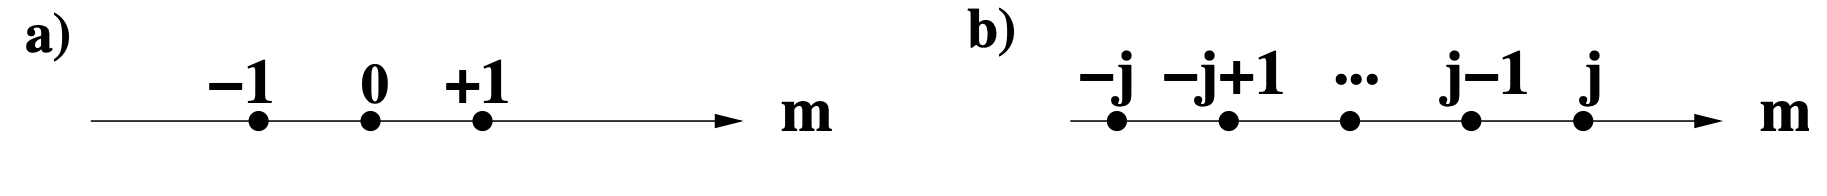
\includegraphics[width=0.75\textwidth]{figures/roots.png}
    \caption{Figure (a) shows the root diagram for the $SU(2)$ Lie algebra. Figure (b) shows the general structure of the weights for irreducible representations of this algebra.}
    \label{fig:su2-root-diagram}
\end{figure}

These relations define the \emph{roots} of the algebra, which is a property independent of the particular representation. However, to understand it better, let's consider the adjoint representation, in which
\begin{subequations}
\begin{align}
    J^{Ad}_3 \ket{J^\pm} &= \pm \ket{J^\pm} \label{appeq:ad1}\\
    J_3^{Ad} \ket{J_3} &= 0 \label{appeq:ad2}\\
\end{align}
\end{subequations}
Focusing on~\eqref{appeq:ad1} and exponentiating it, using~\eqref{appeq:rep-ga} for the left-hand side, we find
\begin{equation}
    g(\xi) \ket{J^\pm} = e^{\pm i \xi J_3} \ket{J^\pm} ,
\end{equation}
which tells us that $\ket{J^\pm}$ transform under the $U(1)$ subgroup generated by the Cartan generator $J_3$, with charges $\pm 1$. Similarly, from~\eqref{appeq:ad2}, $J_3$ has charge $0$. Those charges are called \emph{roots} of the algebra, and in $SU(2)$ case, the charges are $(J_-, J_3, J_+) = (-1,0,1)$. They can be graphically represented in a \emph{root diagram}, as showed in figure~\ref{fig:su2-root-diagram}.

\paragraph{Weights}
Let's now focus on the construction of irreducible representations. The representation space is a vector space spanned by a set of basis vectors. It's then natural to take a basis in which the representative of $J_3$ is diagonal. Then, in this basis, it's natural to label each basis vector by its $J_3$ eigenvalue, that is\footnote{We should write something like $\rho(J_3)$, i.e., we're considering the generator in a particular representation. However, it should be clear from the context whether we're dealing with the abstract generator or its representative in the representation $\rho$.}
\begin{equation}
    J_3 \ket{\mu} = \mu \ket{\mu} .
\end{equation}
Then, $\mu$ are real numbers, since unitary representations of compact groups are given by hermitian operators, which have real eigenvalues. They are the charges of $\ket{\mu}$ under the $U(1)$ transformation generated by the Cartan's generator $J_3$, for an argument similar than the one of the roots. Such charges are called \emph{weights} of the representation, and differently than the roots, depend on the particular representation. In particular, looking at~\eqref{appeq:ad1} and~\eqref{appeq:ad2}, we observe that \emph{roots of the Lie algebra are the weights of the adjoint representation}.

An irreducible representation is essentially defined by giving the set of weights for all basis vector in the representation space. In our case, let's build a finite-dimensional representation, so that $J_3$ has a finite number of eigenstates. Let's pick the state with largest eigenvalue, called the \emph{highest weight} state, with, say, $\mu = j$.

A general property one can prove is that in an \emph{irreducible representation, weights differ by roots}. To show this explicitly in our case, let's start with a state $\ket{\mu}$ and show that the states $J^\pm \ket{\mu}$ are eigenstates of $J^3$ with weight $(\mu \pm 1)$,
\begin{equation}
    J_3 J^\pm \ket{\mu} = (\comm{J_3}{J^\pm} + J^\pm J_3) \ket{\mu} = (\pm J^\pm + \mu J^\pm) \ket{\mu} = (\mu \pm 1) J^\pm \ket{\mu} .
\end{equation}
This means that, if non-vanishing, the states $J^\pm \ket{\mu}$ are part of the basis vectors $\{\ket{\mu}\}$. This shows that there must exists weights which are equal to $\mu \pm 1$, or, in other words, that weights differ by roots. 

Since we called $\ket{j}$ the highest weight state, the basis vectors must be of the form $\ket{j}, \ket{j-1}, \ket{j-2}, \dots$. On the other hand, being the representation finite-dimensional, the previous list should end at a certain point. To see where, let's recall from quantum mechanical courses that
\begin{equation}
\begin{aligned}
    J^- \ket{\mu} &= N_\mu \ket{\mu - 1} \label{appeq:lowering-op}\\
    J^+ \ket{\mu} &= N_\mu \ket{\mu +1},
\end{aligned}
\end{equation}
with normalization constant
\begin{equation}\label{appeq:normalization}
    N_\mu = \sqrt{\frac{1}{2}(j+\mu)(j-\mu+1)} .
\end{equation}

Then, starting from $\ket{\mu = j}$, according to~\eqref{appeq:lowering-op}, we apply the operator $J^-$ to obtain the other states. The representation is consistently finite dimensional if, for some $\mu = q$, we get $J^- \ket{q} = 0$. Looking at the normalization~\eqref{appeq:normalization}, we observe that this is possible for $\mu = -j$, for which
\begin{equation}
    J^-\ket{-j} = 0.
\end{equation}
Further, since $\mu$ differ by integers, $j$ and $-j$ must differ by an integer, so that $j$ must be integer or half odd.

Therefore, we showed that irreducible representations of $SU(2)$ are characterized by the highest weight, which must be an integer or half integer. The representation space is spanned by the basis vectors
\begin{equation}
    \ket{j}, \ket{j-1}, \ket{j-2}, \dots, \ket{-j},
\end{equation}
and is $(2j+1)$-dimensional. All the information of the irreducible representation with highest weight $\mu=j$ is summarized in the weight diagram in figure~\ref{fig:su2-root-diagram}.

%******************** ROOTS AND WEIGHTS FOR GENERAL LIE ALGEBRA *********************
\section{Roots and Weights for general Lie Algebras}
Let's generalize what we saw for $SU(2)$ to a generic group.

\paragraph{Roots}
To put the Lie algebra in the \emph{Cartan-Weyl form}, we pick a \emph{maximal set of mutually commuting hermitian generators}. Here, we're using an abuse of language. Indeed, by abstract hermitian generator, we mean a generator which will be represented by a hermitian operator in any unitary representation. Keeping this in mind, let's call those mutually commuting generators $H_i$, $i = 1, \dots, r$. They generate the \emph{Cartan subalgebra} of the Lie algebra and their number is called the \emph{rank} $r$ of the group. Upon exponentiation, they generate a $U(1)^r$ subgroup of the Lie group.

Then, we rewrite the remaining commutators such that we can easily read off their charges with respect to the $U(1)^r$ generated by the Cartan subalgebra. To do so, we go to the \emph{adjoint representation}, with basis vectors for the representation space given by $\{ \ket{T_a} \}$. We construct the matrices
\begin{equation}
   M_{ab}^{(i)} = \bra{T_a}H_i\ket{T_b}  .
\end{equation}

Since the Cartan generators $H_i$ commute in the abstract algebra, their representative in the adjoint representation, i.e., the matrices $M^{(i)}$, commute. Therefore, they can be simultaneously diagonalized, to get a new basis of vectors $\ket{E_\alpha}$, which are eigenstates of the representative of $H_i$. In particular, we label those states with their eigenvalues $\alpha_i$ with respect to $H_i$, that is\footnote{As before, we should've written something like $Ad(H_i)$, since we're dealing with the representative of the Cartan generators in the adjoint representation $Ad$. However, this should be clear from the context and the use of the braket notation.},
\begin{equation}\label{appeq:eigen-cartan}
    H_i \ket{E_\alpha} = \alpha_i \ket{E_\alpha}.
\end{equation}
Since we're working in the adjoint representation and the above $H_i$ is, more properly, $Ad(H_i)$, let's compare~\eqref{appeq:eigen-cartan} with the relation~\eqref{appeq:adjoint-def}. We conclude that, from the abstract algebra point of view, $E_\alpha$ are some linear combinations of the abstract generators $T_a$, with commutation relation with the abstract $H_i$ given by
\begin{equation}\label{appeq:HE-comm}
    \comm{H_i}{E_\alpha} = \alpha_i E_\alpha .
\end{equation}

In particular, using the hermiticity of $H_i$ and the Jacobi identity, one can show that
\begin{subequations}
\begin{align}
    E^\dagger_\alpha &= E_{-\alpha} \\
    \comm{E_\alpha}{E_{-\alpha}} &= \sum_i \alpha_i H_i \label{eq:prop-1}\\
    \comm{E_\alpha}{E_\beta} &= \begin{cases}
        E_{\alpha + \beta}, \quad \textup{if $\alpha + \beta$ is a root} \\
        0, \quad \textup{otherwise}
    \end{cases}
\end{align}
\end{subequations}

The $r$-dimensional vectors $\alpha$ are called \emph{roots of the Lie algebra}, and they provide the charges of the $E_\alpha$ with respect to the $U(1)^r$ generated by the Cartan subalgebra, as expressed by~\eqref{appeq:HE-comm}

\paragraph{Weights}
To describe irreducible representations, we choose a basis of the representation space where all matrices representing the Cartan generators are diagonal. Then, $H_i$ will be represented by diagonal matrices, and we label the basis vectors by their eigenvalues with respect to those matrices, i.e., by $\{\ket{\mu}\}$, where\footnote{We're using an abuse of notation, again. By $H_i$ we mean $\rho(H_i)$, i.e., the matrices representing $H_i$ in the representation $\rho$.}
\begin{equation}\label{appeq:gen-weight-def}
    H_i \ket{\mu} = \mu_i \ket{\mu}, \quad i = 1, \dots, r.
\end{equation}

The $r$-dimensional vectors $\mu$ are called the \emph{weights of the representation}. The set of weights of a representation characterize the representation itself. As discussed above, while \emph{weights} are properties of the \emph{particular representation}, the \emph{roots} are a property of the \emph{algebra}. Further, the weights of the adjoint representation are the roots of the Lie algebra.

As before, we can prove that \emph{weights differ by roots}. To do so, we start from a generic state $\ket{\mu}$ and show that $E_{\pm \alpha}\ket{\mu}$ is an eigenstate of $H_i$ with eigenvalue $(\mu_i \pm \alpha_i)$, namely
\begin{equation}
    H_i E_{\pm \alpha} \ket{\mu} = ( \comm{H_i}{E_{\pm \alpha}} + E_{\pm \alpha} H_i )\ket{\mu} = ( \pm \alpha_i E_{\pm \alpha} + \mu_i E_{\pm \alpha} )\ket{\mu} = ( \mu_i \pm \alpha_i )E_{\pm\alpha}\ket{\mu}
\end{equation}
where we used~\eqref{appeq:HE-comm} and~\eqref{appeq:gen-weight-def}. This means that, in the representation, there must be a weight given by $(\mu \pm \alpha)$, with corresponding basis state $\ket{\mu \pm \alpha}$.

As in the $SU(2)$ case, one can prove
\begin{equation}\label{appeq:raising-op}
    E_{\pm\alpha} \ket{\mu} = N_{\mu,\pm \alpha} \ket{\mu \pm \alpha},
\end{equation}
and that for some $\mu$ we have $N_{\mu,\pm \alpha} = 0$, which ensures that representations are finite-dimensional. We can further impose additional constraints on the values of the weights $\mu$. The set of allowed irreducible representation and corresponding weights must be analysed case by case.

\paragraph{Relation with \texorpdfstring{$SU(2)$}{SU(2)}}
Each root $\alpha$ defines a $SU(2)$ subalgebra. To see this, let's consider a non-zero root $\alpha = (\alpha_1, \dots, \alpha_r) \neq 0$. One can show that the generators $E_{\pm \alpha}$ and $\sum_i \alpha_i H_i$ form an $SU(2)$ subalgebra of the Lie algebra. In particular, defining
\begin{equation}\label{appeq:su2-subalgebra-def}
    E^\pm = \frac{1}{\abs{\alpha}} E_{\pm \alpha}, \quad E_3 = \frac{1}{\abs{\alpha}^2} \sum_i \alpha_i H_i ,
\end{equation}
one can prove they satisfy the $SU(2)$ algebra commutation relations in the Cartan-Weyl form, namely
\begin{equation}\label{appeq:su2-subalgebra}
     \comm{E_3}{E^\pm} = \pm E^\pm, \quad \comm{E^+}{E^-} = E_3 .
\end{equation}

\begin{mdframed}
\begin{innerproof}
    Using~\eqref{appeq:su2-subalgebra-def} and~\eqref{appeq:eigen-cartan} we can compute
    \begin{equation}
        \comm{E_3}{E^\pm} = \frac{1}{\abs{\alpha}^3} \sum_i \alpha_i \comm{H_i}{E_{\pm\alpha}} = \pm \frac{E_{\pm\alpha}}{\abs{\alpha}} = \pm E^\pm .
    \end{equation}
    Further, using~\eqref{appeq:su2-subalgebra-def} and~\eqref{eq:prop-1} we can compute
    \begin{equation}
        \comm{E^+}{E^-} = \frac{1}{\abs{\alpha}^2} \comm{E_{+\alpha}}{E_{-\alpha}} = \frac{1}{\abs{\alpha}^2} \sum{\alpha_i H_i} = E_3 ,
    \end{equation}
    as claimed.
\end{innerproof}
\end{mdframed}

This allows us to organize generic Lie algebra weights into $SU(2)$ irreducible representations. In particular, let's start with a generic weight $\mu$ and apply the operators $E^{\pm}$. By means of~\eqref{appeq:raising-op}, we obtain
\begin{subequations}
\begin{align}
    E^+ \ket{\mu} = \frac{E_{+\alpha}}{\abs{\alpha}} \ket{\mu} = \frac{N_{\mu, +\alpha}}{\abs{\alpha}} \ket{\mu + \alpha} ,\\
    E^- \ket{\mu} = \frac{E_{-\alpha}}{\abs{\alpha}} \ket{\mu} = \frac{N_{\mu, -\alpha}}{\abs{\alpha}} \ket{\mu - \alpha} .\\
\end{align}
\end{subequations}

Therefore, continuous applications of the operators $E^\pm$, given any weight $\mu$, leads to states proportional to $\ket{\mu \pm \alpha}$, with $k \in \N_0$. In particular, for $p,q \in \N$,
\begin{subequations}
    \begin{align}
        (E^+)^p \ket{\mu} = \left(\frac{E_{+\alpha}}{\abs{\alpha}}\right)^p \ket{\mu} = \frac{\prod_{l=0}^{p-1} N_{\mu + l\alpha, +\alpha}}{(\abs{\alpha})^p} \ket{\mu + p \alpha} \propto \ket{\mu + p \alpha},\\
        (E^-)^q \ket{\mu} = \left(\frac{E_{-\alpha}}{\abs{\alpha}}\right)^q \ket{\mu} = \frac{\prod_{l=0}^{q-1} N_{\mu - l\alpha, -\alpha}}{(\abs{\alpha})^q} \ket{\mu - q \alpha} \propto \ket{\mu - q \alpha} .\\
    \end{align}
    \end{subequations}

From the $SU(2)$ Cartan-Weyl algebra point of view, with respect to $E_3$ and $E^\pm$, the highest weight state is defined by $E^+ \ket{\mu + p\alpha} = 0$ and $E^- \ket{\mu - q \alpha} = 0$. They must be eingenstates of the Cartan generator $E_3$ as well, and in particular, we have
\begin{subequations}
\begin{align}
    E_3 \ket{\mu + p \alpha} = \left( \frac{\mu \cdot \alpha}{\abs{\alpha}^2} + p \right) \ket{\mu + p \alpha} \\
    E_3 \ket{\mu - q \alpha} = \left( \frac{\mu \cdot \alpha}{\abs{\alpha}^2} - q \right) \ket{\mu - q \alpha} \\
\end{align}
\end{subequations}

\begin{mdframed}
\begin{innerproof}
    For $k \in \N$, using the definition~\eqref{appeq:su2-subalgebra-def} and the eigenstate equation~\eqref{appeq:gen-weight-def}
    \begin{equation*}
    \begin{split}
        E_3 \ket{\mu \pm k \alpha} &= \frac{1}{\abs{\alpha}^2} \sum_i \alpha_i H_i \ket{\mu \pm k \alpha} = \frac{1}{\abs{\alpha}^2} \sum_i \alpha_i (\mu_i \pm k \alpha_i) \ket{\mu \pm k \alpha}\\ 
        &= \left( \frac{\alpha \cdot \mu}{\abs{\alpha}^2} \pm k \right) \ket{\mu \pm k \alpha} .
    \end{split}
    \end{equation*}
   Taking $k = p$ or $k= -q$ concludes the proof.
\end{innerproof}
\end{mdframed}

Recalling that the highest and lowest weight state for $SU(2)$ are $\ket{j}$ and $\ket{-j}$, such that $E_3 \ket{\pm j} = \pm j \ket{\pm j}$, we impose
\begin{subequations}
\begin{align}
    E^+ \ket{\mu + p\alpha} &\overset{\mathrm{!}}{=} E^+ \ket{j} = 0  \implies j = \frac{\alpha \cdot \mu}{\abs{\alpha}^2} + p, \\
    E^- \ket{\mu - q\alpha} &\overset{\mathrm{!}}{=} E^- \ket{-j} = 0 \implies -j = \frac{\alpha \cdot \mu}{\abs{\alpha}^2} -q . 
\end{align}
\end{subequations}
Collectively those formulas imply
\begin{equation}\label{eq:master-formula}
    \frac{\alpha \cdot \mu}{\abs{\alpha}^2} = -\frac{1}{2}(p-q) ,
\end{equation}
which is knows as \emph{master formula}.

This allows us to construct irreducible representations in the following way. First, we can define a \emph{positive vector} in the weight/root space as a vector $v$ whose first non-zero component is positive. Therefore, if $v_1 \neq 0$, then $v > 0$ if $v_1 > 0$. Otherwise, if $v_1 = 0$ and $v_2 \neq 0$, then $v > 0$ if $v_2 > 0$ and so on. Then, given two weight/root space vectors $v$ and $\omega$, we can define a \emph{positive direction} through the ordering for which $v > \omega$ if $v - \omega > 0$, i.e., if $v-\omega$ is a positive vector, as defined above.

Then, turning to weights, we can define the \emph{highest weight} $\mu_0$ of a representation as the weight such that $\mu_0 > \mu$ for any other weight $\mu$.

Moreover, for what concern roots, we can split the non-zero ones into the set of \emph{positive roots} and of \emph{negative roots}, as described above. For a positive roots $\alpha > 0$, $E_\alpha$ are \emph{raising operators}, while $E_{-\alpha}$ are \emph{lowering operators}. Then, the highest weight vector is characterized by the fact that it is annihilated by the raising operators, otherwise we'd get states $\ket{\mu_0 + \alpha}$, with weight higher than $\ket{\mu_0}$.

Finally, the whole representation is built by applying lowering operators to the highest weight state, in all possible inequivalent ways. At a certain point we'll find zero, states form representations of $SU(2)$ associated to each $\alpha$, and such representation are finite-dimensional.

%******************** SU(3) *********************
\section{\texorpdfstring{$SU(3)$}{SU(3)}}
Instead of giving the commutation relations of the $SU(3)$ algebra, all the relevant information is provided by the root diagram, showed in figure~\ref{fig:su3-root-diagram}.

\begin{figure}
    \centering
    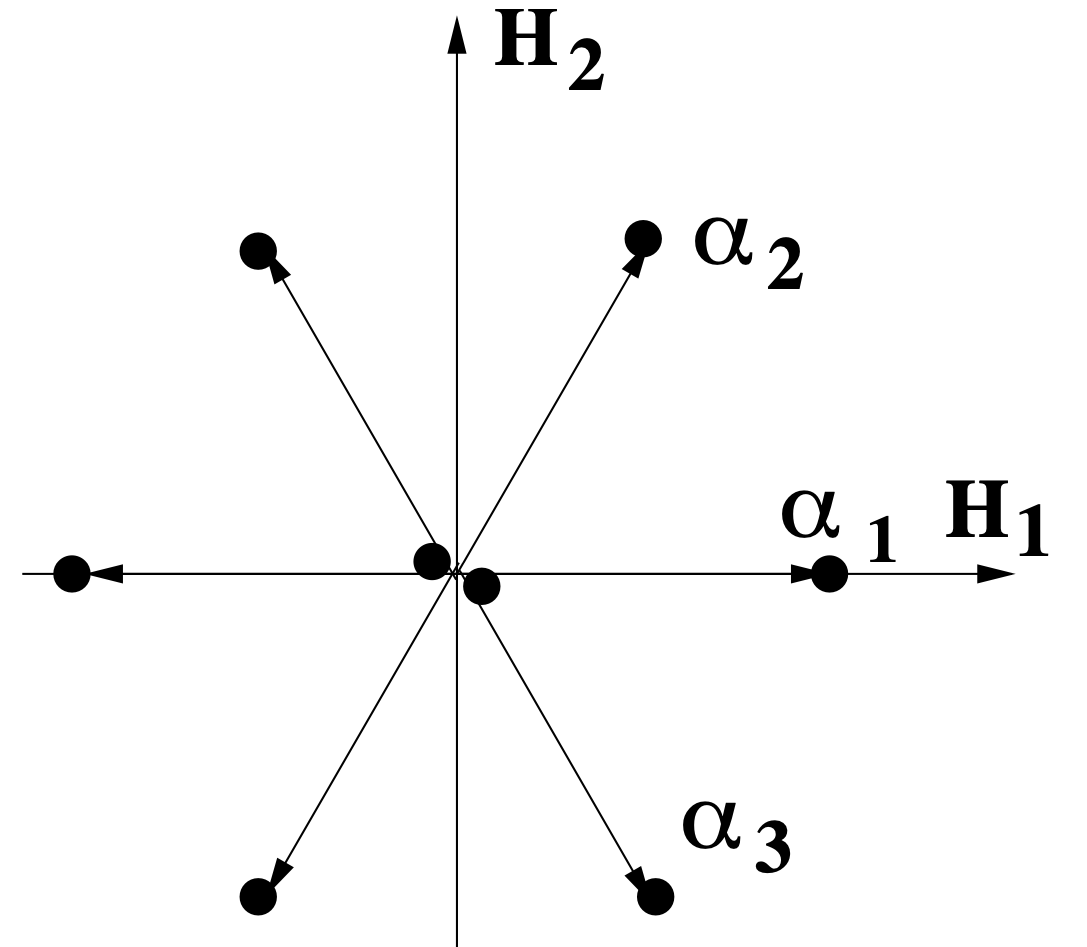
\includegraphics[width=0.3\textwidth]{figures/su3-root.png}
    \caption{The root system of the $SU(3)$ Lie algebra. The positive roots are $\alpha_1 = (1,0)$, $\alpha_2 = (1/2, 1/(2\sqrt{3}))$, $\alpha_3 = (1/2, -1/(2\sqrt{3}))$. The two roots at $(0,0)$ correspond to the Cartan generators.}
    \label{fig:su3-root-diagram}
\end{figure}

We can observe that the rank is $2$, which means the Cartan subalgebra is spanned by two generators $H_1$ and $H_2$, which are mutually commuting. The remaining $8$ generators are labelled by $E_\alpha$ and $E_{-\alpha}$, for $\alpha = (1,0), (1/2, 1/(2\sqrt{3})), (1/2, -1/(2\sqrt{3}))$, with commutation relations
\begin{equation}
    \comm{H_i}{E_{\pm \alpha}} = \pm \alpha_i E_{\pm \alpha} .
\end{equation}
The $SU(2)$ subalgebras for different $\alpha$ correspond, graphically, to the lines along which the roots reproduce the root diagram of $SU(2)$, in figure~\ref{fig:su2-root-diagram}.

Further, instead of writing explicit matrices providing a particular representation of the $SU(3)$ algebra, we can instead provide the weight diagram of the corresponding representation. As an example, the fundamental representation has complex dimension $3$, and the generators are represented by $8$ \emph{Gell-Mann matrices}. Upon exponentiation, the group elements are represented by $3 \times 3$ unitary matrices.

\begin{figure}
    \centering
    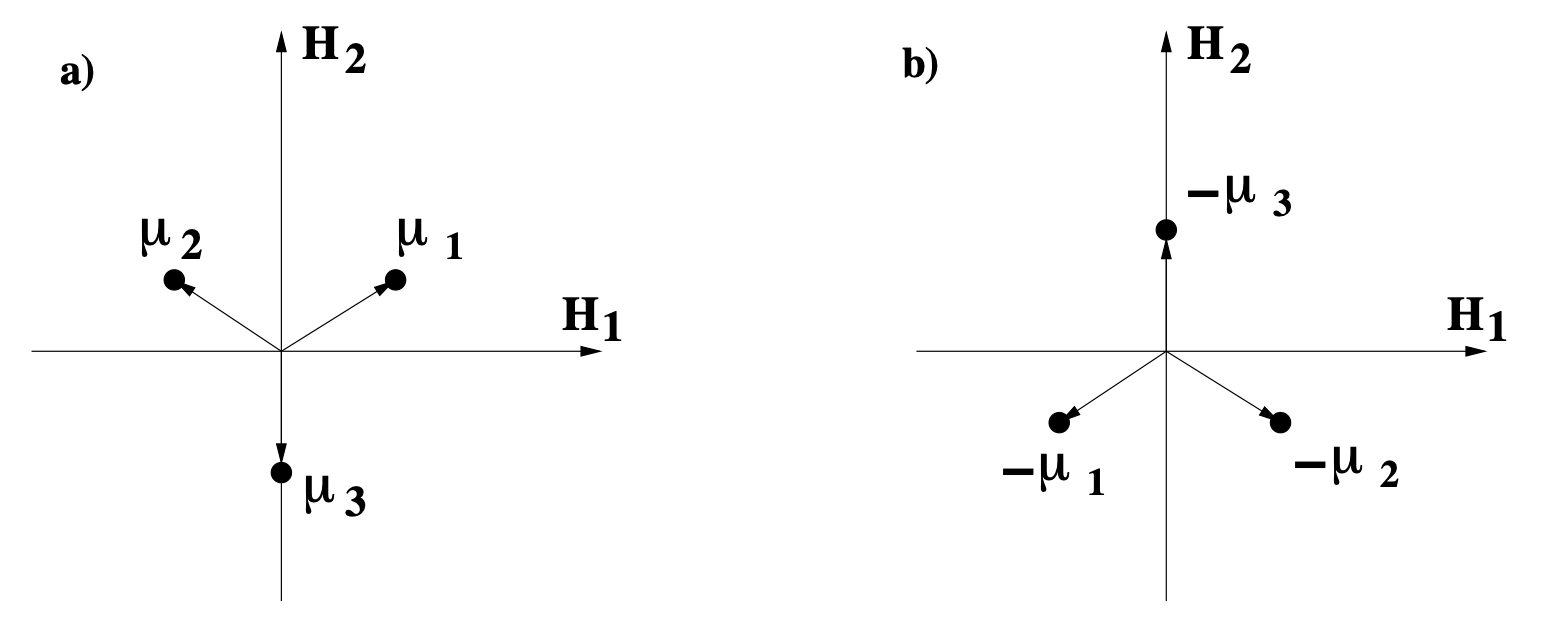
\includegraphics[width=0.7\textwidth]{figures/su3-weights.png}
    \caption{The weight diagram for the fundamental (a) and the antifundamental (b) representations of $SU(3)$. In particular $\mu_1 = (1/2, 1/(2\sqrt{3}))$, $\mu_2 = (-1/2, 1/(2\sqrt{3}))$ and $\mu_3 = (0, -1/\sqrt{3})$.}
    \label{fig:weight-su3-fund}
\end{figure}

This representation can be equivalently descibed by the weights in figure~\ref{fig:weight-su3-fund}. The action of the Cartans on the states $\ket{\mu = (\pm 1/2, 1/(2\sqrt{3})), (0,-1/\sqrt{3})}$ is
\begin{equation}
    H_i \ket{\mu} = \mu_i \ket{\mu} ,
\end{equation}
while the action of non-zero root generators $E_\alpha$ is
\begin{equation}
    E_\alpha \ket{\mu} = N_{\mu,\alpha}\ket{\mu + \alpha} .
\end{equation}

Notice that the states form representations under the $SU(2)$ subalgebras of the non-zero roots. That is, weights along lines parallel to the root diagram of the corresponding $SU(2)$ subgroup differ by the corresponding root.

The construction of irreducible representations is as follows. The highest weight is $\ket{\mu_1} = \ket{(1/2, 1/(2\sqrt{3}))}$, and is annihilated by the positive roots $\alpha_1 = (1,0)$, $\alpha_2 = (1/2, 1/(2\sqrt{3}))$ and $\alpha_3 = (1/2, -1/(2\sqrt{3}))$. The remaining states are obtained as
\begin{equation}
\begin{aligned}
    E_{-\alpha_1} \ket{(1/2,1/(2\sqrt{3}))} &\simeq \ket{(-1/2,1/(2\sqrt{3}))} ,\\
    E_{-\alpha_3} \ket{(1/2, 1/(2\sqrt{3}))} & \simeq \ket{0, -1/\sqrt{3}} .
\end{aligned}
\end{equation}

The conjugate representation, the antifundamental, which is obtained by minus the transposed Gell-Mann matrices, has weights opposite to those of the fundamental. Namely, conjugation of the representation flips the charges of objects. The weights are shown in figure~\ref{fig:weight-su3-fund}.

%*********************** DYNKIN DIAGRAMS *************************
\section{Dynkin Diagrams}
\paragraph{Angle of Roots}
Recall the master formula~\eqref{eq:master-formula}. It gives us a constraint of the weights, by requiring that $\ket{\mu + k\alpha}$ is a representation of $SU(2)_\alpha$, where $k \in \N$. We can apply it to the adjoint representation, where the weights $\mu$ are roots. Then, we can require that the states $\ket{\beta + k \alpha}$ form a representation of $SU(2)_\alpha$, and that the states $\ket{\alpha + k \beta}$ form a representation of $SU(2)_\beta$, getting
\begin{equation}
    \frac{\alpha \cdot \beta}{\abs{\alpha}^2} = - \frac{1}{2} m , \quad \frac{\beta \cdot \alpha}{\abs{\beta}^2} = - \frac{1}{2} m', \quad m, m' \in \Z.
\end{equation}

Then, we obtain a constraint on the relative angle of the roots, namely
\begin{equation}
    \cos^2 \theta_{\alpha\beta} \equiv \frac{(\alpha\cdot\beta)^2}{\abs{\alpha}^2\abs{\beta}^2} = \frac{mm'}{4}.
\end{equation}
The angle is constraint to be $0,30,45,60,90,120,135,150,\textup{or} \, 180$ degrees.

\paragraph{Simple Roots}
We define a \emph{simple root} as a positive root which cannot be written as a sum of positive roots with positive coefficients. One can show that the set of simple roots of an algebra is linearly independent and form a basis of the root space.

Further, one can see that the angle of simple roots is more constraint. To show this, let's first notice that if $\alpha$ and $\beta$ are simple roots, then $\alpha - \beta$ is \emph{not} a root. Indeed, if it were a root, it would be either positive or negative. If it is positive, then $\alpha = \beta + (\alpha - \beta)$ contradicts the fact that $\alpha$ is simple, while if it is negative, then $\beta = \alpha - (\alpha - \beta)$ contradicts that $\beta$ is simple.

Going in the adjoint representation, $E_{-\alpha}$ must annihilate $\ket{E_\beta}$, which makes it the lower weight state $\ket{-j}$ for the subalgebra $SU(2)_\beta$. Otherwise, $E_{-\alpha} \ket{E_\beta} \propto \ket{E_{\beta - \alpha}}$, but this is not possible since $\beta - \alpha$ is not a root. Then, with a similar argument used to derive the master formula~\eqref{eq:master-formula}, and inverting the roles of $\alpha$ and $\beta$, we get
\begin{equation}
    2 \frac{\alpha \cdot \beta}{\abs{\alpha}^2} = - p, \quad 2 \frac{\beta \cdot \alpha}{\abs{\beta}^2} = -p'  \quad p,p' \in \N .
\end{equation}

Therefore,
\begin{equation}\label{appeq:cosine}
    \cos \theta_{\alpha\beta} = -\frac{1}{2} \sqrt{pp'},
\end{equation}
which constraints the angles between simple roots to be $90,120,135,\text{or}\,150$ degrees.

\paragraph{Cartan Classification}
The \emph{relative lengths} and \emph{relative angles} are invariants of the set of simple roots. Using that simple roots provides a basis of the root space, one can recover the complete system of roots using the invariants. Then, the problem of classifying the Lie algrebras is reduced to the problem of classifying sets of $r$ linearly independent vectors in $r$-dimensional space with non-positive integer values of $2\frac{\alpha \cdot \beta}{\abs{\alpha}^2}$.

Before moving on, let's notice that if we have two systems of simple roots, of dimensions $r_1$ and $r_2$, we can combine them to form a $(r_1 + r_2)$-dimensional simple root system, by joining orthogonally the two initial systems. We're interested in root systems which can't be split into orthogonal subsystems. This is related to the concept of invariant subalgebras.

Given an algebra $A$, an \emph{invariant subalgebra} is a subalgebra such that the commutator of any element of $B$ with any element of $A$ is still in $A$. Upon exponentiation, Lie algebras with invariant subalgebras lead to \emph{non-simple} groups, which are groups which split as product of groups, like $G = G_1 \times G_2$. A Lie algebra without invariant subalgebras are called \emph{simple Lie algebra}.

So, in principle, we're interested in classifying simple groups and simple Lie algebras, since the others can be derived from them. One can further show that Lie algebras with invariant subalgebras manifest as root systems which split into two othogonal subsystems. Hence, we're interested in classifying \emph{simple root systems}, which don't have such subsystems. Any other system can be obtained by adjunction. 

\begin{figure}
    \centering
    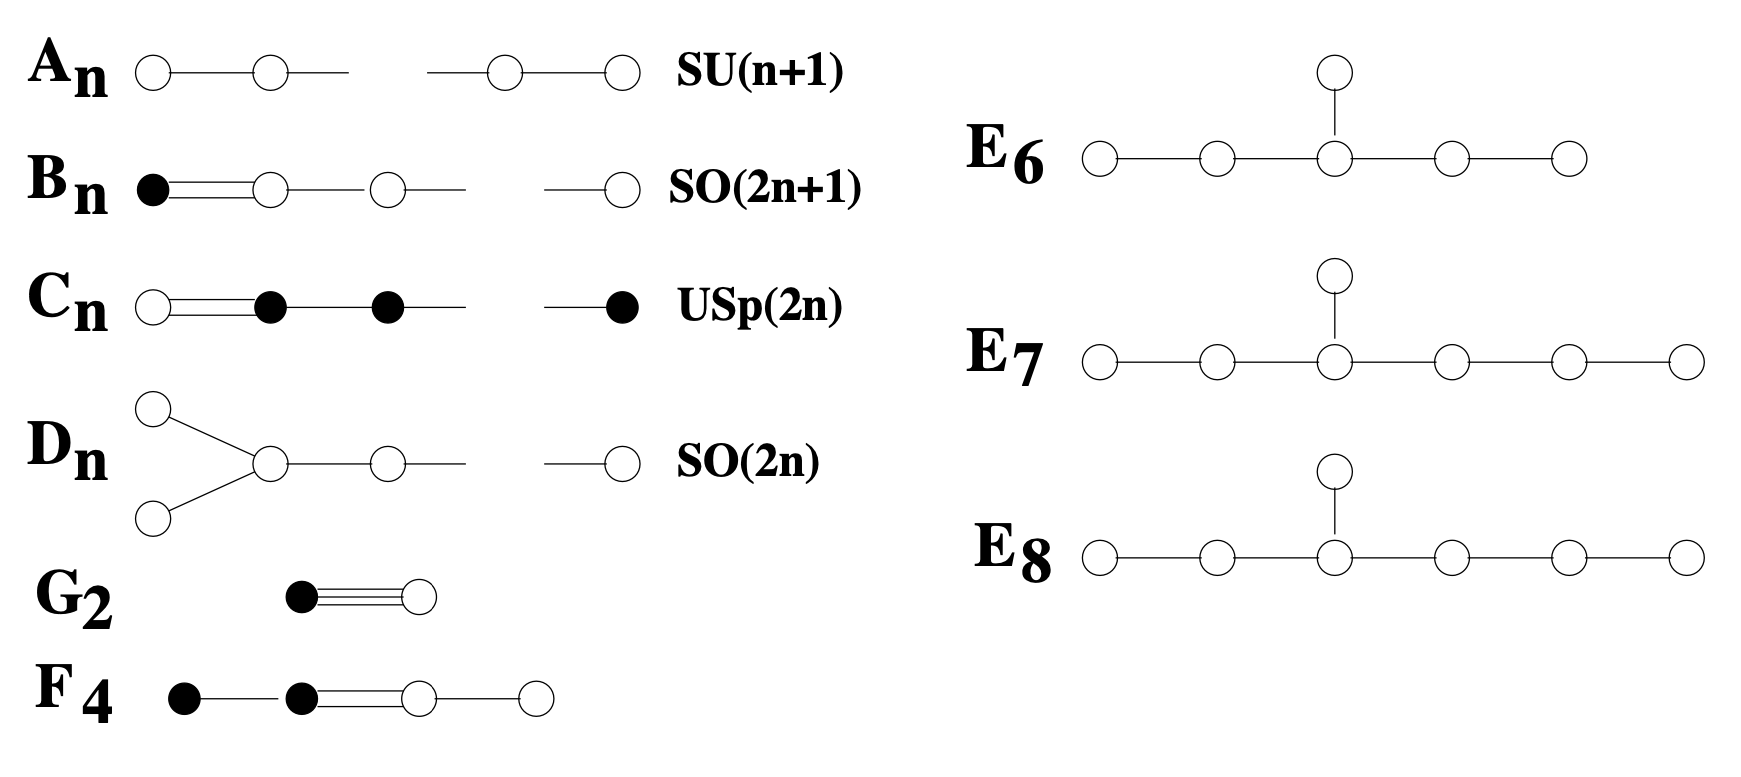
\includegraphics[width=0.75\textwidth]{figures/dynkin.png}
    \caption{Dynkin diagrams for simple Lie algebras. There are four infinite series (labelled by a positive integer $r$, giving the number of nodes), and some exceptional algebras. Notice that for small rank some algebras are isomorphic and have the same Dynking diagram (e.g., $A_3 = D_3$, namely $SU(4) \simeq SO(6)$). The groups arising from the $A$, $B$, $C$, and $D$ series were known in classical mathematics before Cartan and are known as classical Lie groups, they are listed to the right of the corresponding diagram.}
    \label{fig:dynkin}
\end{figure}

The problem of classifying simple root systems of this kind has been solved. The result, called the \emph{Cartan classification}, can be recast in giving the relative lengths and angles between the simple roots. This is conveniently represented in the \emph{Dynkin diagram}. The classification of Dynkin diagrams for simple Lie algebras is given in figure~\ref{fig:dynkin}. 

The rules to obtain the simple root system from the diagram are as follows:
\begin{itemize}
    \item each node corresponds to a simple root. Hence, the number of nodes is the rank of the Lie algebra/group;
    \item the number of lines joining two nodes gives us the angle between the two simple roots: no line means $90$°, one line means $120$°, two lines means $135$°, three lines means $150$°;
    \item dark nodes correspond to shorter roots. The relative lengths can be found from eq.~\eqref{appeq:cosine}.
\end{itemize}

Clearly, Dynking diagrams corresponding to non-simple algebras are obtained by adjoining in a disconnected way Dynkin diagrams for simple algebras, so that we adjoin orthogonally the two subsystems of simple roots.

%*********************** SU(K) GROUP *************************
\section{The Group \texorpdfstring{$SU(k)$}{SU(k)}}
\paragraph{Roots}
Although $SU(k)$ (or its algebra $A_{k-1})$ has rank $k-1$, it is convenient and easier to describe its roots as $k$-dimensional vectors, which lie on an $(k-1)$-plane. Besides the $k-1$ zero roots associated to the Cartan generators, the non-zero roots are given by the $k$-dimensional vectors  
\begin{equation}
    (\underline{+,-,0,\dots,0}),
\end{equation}
where $+,-$ denote $+1, -1$, and where underlining means permutation, namely the $+$ and $-$ can be located in any (non-coincident) positions. Note that all roots satisfy one relation $\sum_{i=1}^n v_i = 0$, so they live in a $(k-1)$-plane $\Pi$ in $\R^n$. There are a total of $k^2-1$ roots, which is the number of generators of $SU(k)$.

Fixing a basis within the $(k-1)$-plane it is straightforward to read out the roots as $(k-1)$-dimensional vectors. The picture of the root system of $SU(3)$ in this language is given in figure~\ref{fig:su3-root-system}.

\begin{figure}
    \centering
    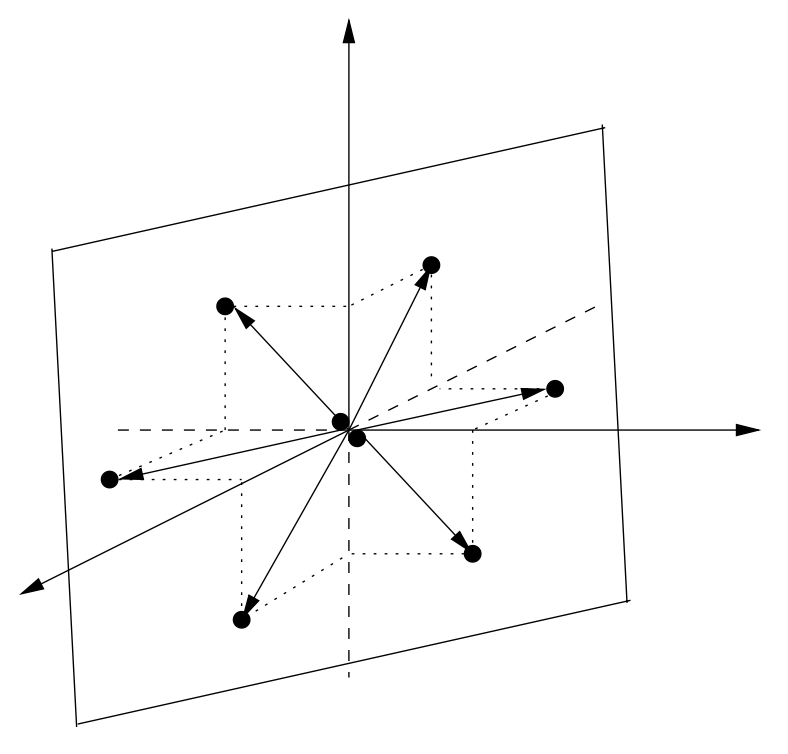
\includegraphics[width=0.4\textwidth]{figures/su3-root-system.png}
    \caption{The root system of $SU(3)$ described as a set of vectors lying in a $2$-plane in $3$-dimensional space.}
    \label{fig:su3-root-system}
\end{figure}

The extra direction in the diagram can be regarded as associated to the extra $U(1)$ generator in $U(k) = SU(k) \times U(1)$. Hence, $SU(k)$ weight diagrams embedded in $(k-1)$-planes parallel to $\Pi$ but not passing through the origin are associated to states which, in addition to being in a representation of $SU(k)$, also carry some charge under the additional $U(1)$.

\paragraph{Weights}
A familiar representation is the fundamental representation. The corresponding weights, given as $k$-dimensional vectors but inside the $(k-1)$-plane $\Pi$ are,
\begin{equation}\label{appeq:fund-weights}
    \frac{1}{n} (\underline{n-1, -1, \dots, -1}) .
\end{equation}
Notice that weights differ by roots, so application of generators associated to non-zero roots relate states with different weights (or give zero if they take us out of the representation).
In situations where the gauge group is $U(k)$, so there is an additional $U(1)$ generator, the fundamentals of $SU(k)$ may carry some charge, so the weights satisfy the relation $\sum_{i=1}^n v_i = q$, for some non-zero constant $q$ giving (up to normalization) the charge under the additional $U(1)$. Very often one finds fundamentals from weights of the form
\begin{equation}\label{appeq:fund1}
    (\underline{+,0,\dots,0}),
\end{equation}
or
\begin{equation}\label{appeq:fund2}
    \frac{1}{2} (\underline{+,-,dots,-}).
\end{equation}

Notice that the weights~\eqref{appeq:fund-weights} can be written as
\begin{equation}
    (\underline{+,0,\dots,0}) - (1/n, \dots, -1/n),
\end{equation}
where the second term removes the piece corresponding to the additional $U(1)$ charge. By abuse of language, we will often use things expressions like~\eqref{appeq:fund1} or~\eqref{appeq:fund2} to denote the fundamental even in situations where there is no additional $U(1)$, removing implicitly the piece corresponding to this charge.

The weights for the antifundamental representation are the opposite to those for the fundamental, namely
\begin{equation}
    (\underline{-,0,\dots,0}).
\end{equation}
By this, we mean
\begin{equation}
    \frac{1}{n} (\underline{-(n-1),1,\dots,1}),
\end{equation}
or any other shifted version, with the understanding that the additional $U(1)$ charge should be removed.

Other representations can be obtained by taking tensor products of the
fundamental, and the corresponding weights are obtained by adding the weights of the fundamental representation.

For instance, the two-index antisymmetric representation has $k(k-1)/2$ weights
\begin{equation}
    (\underline{+,+,0,\dots,0}),
\end{equation}
while the two-index symmetric representation has $k(k+ 1)/2$ weights
\begin{equation}
    (\underline{+,+,0,\dots,0}), \quad (\underline{\pm 2, 0, \dots, 0}).
\end{equation}
They are obtained by adding two times weights of the fundamental representation in a way consistent with antisymmetry or symmetry of the representation.

It is straightforward to derive familiar facts like the equivalence of the antifundamental representation and the $(k-1)$-index antisymmetric representation. They have the same weights.


%*********************** SO(2r) GROUP *************************
\section{The Group \texorpdfstring{$SO(2r)$}{SO(2r)}}
\paragraph{Roots}
Besides the $n$ zero roots, the non-zero roots for the $D_r$ Lie algebra are given by the $r$-dimensional vectors
\begin{equation}
    (\underline{\pm,\pm,0,\dots,0}),
\end{equation}
meaning that the $+$ and $-$ can be choses arbitrarily in any non-coincident position. The total number of roots is $2r(2r-1)/2$.

\begin{figure}
    \centering
    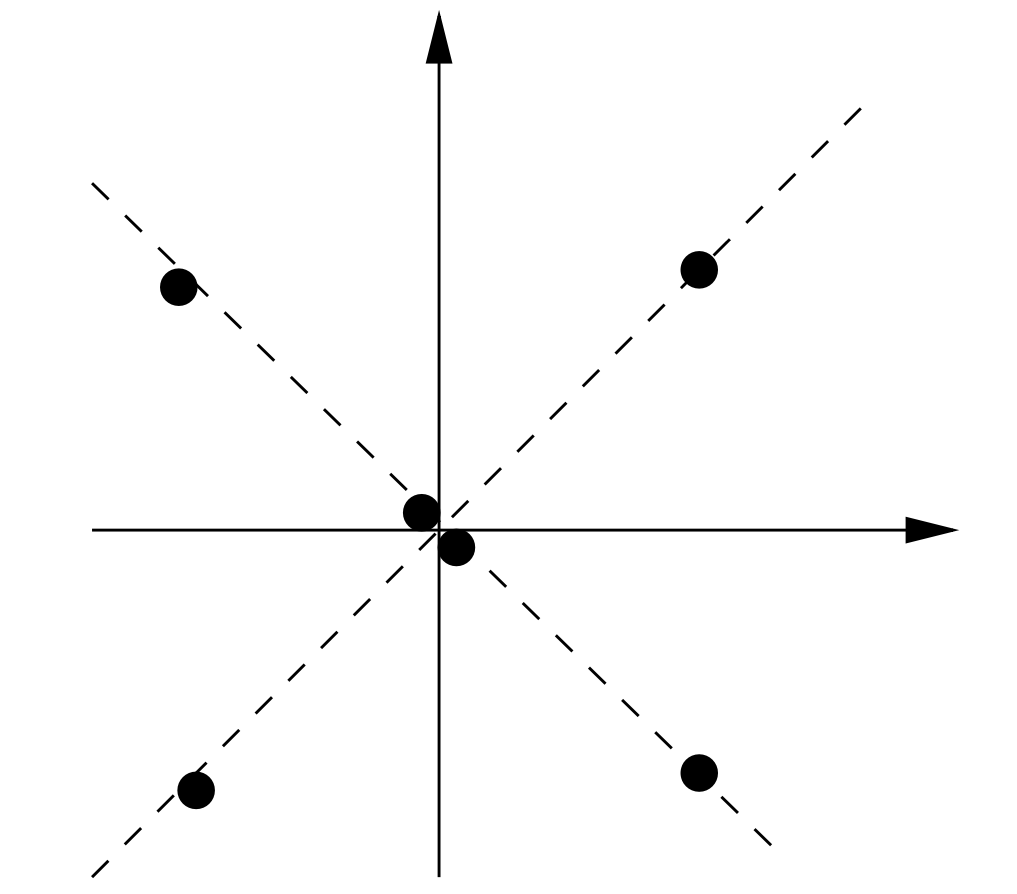
\includegraphics[width=0.35\textwidth]{figures/so4-root-system.png}
    \caption{ Root diagram for $SO(4)$. In fact, it splits as two orthogonal $SU(2)$ root systems.}
    \label{fig:so4-root-system}
\end{figure}

The root system of $SO(4)$ is shown in figure~\ref{fig:so4-root-system}. The fact that there are
two subsets of orthogonal roots means that there are invariant subalgebras. In fact, $SO(4) \simeq SU(2) \times SU(2)'$, with non-zero roots of the latter being given by
\begin{equation}
    SU(2): (+,+),\,(-,-), \quad SU(2)': (+-),\,(-+) .
\end{equation}
Notice also that the Dynkin diagram for $D_2$ are two disconnected nodes, so is the same as two $A_1$ Dynkin diagrams.

It is important to notice that the root system of $SO(2r)$ contains the roots of $SU(r)$, so by exponentiation the group $SO(2r)$ contains a subgroup $SU(r)$.

\paragraph{Weights}
An important representation is the \emph{vector representation}, which is $2r$-dimensional and has weights
\begin{equation}
    (\underline{\pm,0,\dots,0}).
\end{equation}
Notice that it is a real representation, since its conjugate has opposite weights, but the representation (as a whole) is invariant under such change.

When the group is regarded as the group of rotational isometries of a $2r$-dimensional euclidean space, the vector representation in which vectors of this space transform.

More representations can be obtained by taking tensor products of the vector representation. These are the representations under which tensors in the euclidean space transform under rotations.

There are some additional representations which cannot be obtained from tensor products of the vector representation. These are the spinor representations. For $D_r$ there are two inequivalent irreducible spinor representations, both with dimension $2^{r-1}$, and weights
\begin{equation}
\begin{aligned}
    \textup{spinor}: \quad  &\left(\pm\frac{1}{2}, \dots, \pm \frac{1}{2}\right), \quad \textup{$\#-=$even}, \\
    \textup{spinor'}: \quad &\left(\pm\frac{1}{2}, \dots, \pm \frac{1}{2}\right), \quad \textup{$\#-=$odd}.
\end{aligned}
\end{equation}
These spinor representations are said to have different chirality

%*********************** CLIFFORD ALGEBRA *************************
\section{Spinor Representations and Clifford Algebra}
There is a canonical and very useful way to describe the spinor representations of $SO(2r)$, related to representations of Clifford algebras.

Consider the algebra of objects $\Gamma^i$, $i = 1, \dots, 2r$, satisfying
\begin{equation}\label{appeq:clifford}
    \{\Gamma^i, \Gamma^j\} = 2 \delta_{ij}.
\end{equation}
It is called a Clifford algebra.

The important point is that this algebra is invariant under the group of transformations
\begin{equation}
    \Gamma'^i = R^i_j \Gamma^j,
\end{equation}
where $R$ is a $2r\times2r$ orthogonal matrix. This group is precisely $SO(2r)$, and we have found it acting on the set of $\Gamma^i$ in the fundamental representation.

The fact that the Clifford algebra~\eqref{appeq:clifford} has an $SO(2r)$ invariance menas that any representation of the Clifford algebra must also form a representation of $SO(2r)$. In fact, given a hermitian matrix representation for the $\Gamma^i$, the hermitian matrices $J^{ij} = -\frac{i}{4}\comm{\Gamma^i}{\Gamma^j}$ can be seen to form a (possibly reducible) hermitian matrix representation of the $SO(2r)$ algebra, which is
\begin{equation}
    \comm{J^{ij}}{J^{kl}} = i \left( \delta^{ik} J^{jl} + \delta^{jl} J^{ik} - \delta^{il} J^{jlk} - \delta^{jk} J^{il} \right)
\end{equation}

So our purpose is to build a representation of the Clifford algebra, and the resulting representations of $SO(2r)$. The standard technique to build a representation of the Clifford algebra is to form linear combinations of the $\Gamma^i$ which can act as raising and lowering operators. We define
\begin{equation}
    A_a = \frac{1}{\sqrt{2}} (\Gamma_{2a}+i \Gamma_{2a-1}), \quad A^\dagger_a = \frac{1}{\sqrt{2}} (\Gamma_{2a}-i \Gamma_{2a-1}), \quad  a = 1, \dots, r .
\end{equation}
They satisfy the relations
\begin{equation}
    \{ A^\dagger_a, A^\dagger_b \} = \{ A_a, A_b \} = 0, \quad \{A^\dagger_a, A_b\} = \delta_{ab} .
\end{equation}
So they behave as fermionic oscillator ladder operators. Notice that in this language only an $SU(r)$ invariance is manifest, with the $A^\dagger_a$, $A_a$ transforming in the fundamental and antifundamental representations, respectively.

To build a representation of the Clifford algebra, we introduce a “ground-state” for the harmonic oscillator
\begin{equation}
    A_a \ket{0} = 0.
\end{equation}
The representation is built by applying raising operators to this “ground-state” in all possible inequivalent ways. We have
\begin{equation}\label{appeq:states-harmonic-osc}
\begin{aligned}
    \textup{states} \quad &\textup{numbers} \\
    \ket{0} \quad &1  \\
    A^\dagger_a\ket{0} \quad &r \\
    A^\dagger_a A^\dagger_b \ket{0} \quad &r(r-1)/2 \\
    \dots \quad &\dots \\
    A^\dagger_{a_1} \dots A^\dagger_{a_k} \ket{0} \quad &\binom{r}{k} \\
    \dots \quad &\dots \\
    A^\dagger_1 \dots A^\dagger_r \ket{0} \quad &1
\end{aligned}
\end{equation}
The bunch of $\binom{r}{k}$ states arising from applying $k$ operators to the ground-state clearly forms a $k$-index completely antisymmetric tensor representation of the $SU(r)$ invariance group.

The total number of states is $2^r$. Constructing the Lorentz generators, it is possible to check that the weights are of the form
\begin{equation}
    \left( \pm \frac{1}{2}, \dots, \frac{1}{2} \right).
\end{equation}
Moreover, it is easy to realize that the weights among the above with has $k +1/2$'s correspond to the weights of a $k$-index completely antisymmetric tensor representation of $SU(r)$, in agreement with our above statement.

The above weights therefore define a representation of the $SO(2r)$ group (although only $SU(r)$ invariance was manifest in intermediate steps). Now, this representation is reducible. Recalling that the $SO(2r)$ generators are constructed with products of two $\Gamma^i$'s, it is clear that they are unable to relate states~\eqref{appeq:states-harmonic-osc} with even number of $\Gamma$'s to states with odd number of $\Gamma$'s. 

More formally, one can introduce the chirality operator $\Gamma = \Gamma^1 \dots \Gamma^{2r}$ which commutes with all $SO(2r)$ generators (and anticommutes with the $\Gamma^i$), and can be used to distinguish the two subsets of states.

This means that the $2^r$-dimensional representation is reducible into two $2^{r-1}$-dimensional irreducible representations.